%% Einfügen der Präambel
%% Ermöglicht die Kompilierung durch Sublime Text von jeder *.tex Datei aus.
%!TEX root = main.tex

%%% PDF Erstellung mit Glossar
%%% 1 . Kompilieren durch Sublime Tex
%%% 2. Folgende Befehle im Terminal eingeben
%%%	pdflatex main
%%%	makeindex -s main.ist -t main.alg -o main.acr main.acn
%%%	makeindex -s main.ist -t main.glg -o main.gls main.glo
%%%	makeindex -s main.ist -t main.slg -o main.syi main.syg
%%%	pdflatex main

%%% Für schöneren Index wird die Datei index.ist benötigt. Im Terminmal "makeindex -g -s index.ist main" ausführen danach normal kompilieren (davor vielleicht auch schon mal).

%%% Bei Beschreibungen für [] und {}: Durch Komma getrennte Beschreibungen zeigen auf die in [] optionalen Parameter. Nach Semikolon Beschreibungen für den Parameter in {}. Ohne Kommatas = allgemeine Beschreibung. Nur kommatas = Beschreibung der Optionen in [] oder {}.

%% Schriftgröße 12, Format A4, Aufnahme des Abbildungsverzeichnis ins Inhaltsverzeichnis, Aufnahme des Literaturverzeichnis ins Inhaltsverzeichnis, Kapitel und Inhaltsverzeichnis u.a. beginnen auf der rechten Seite, Richtige Seitenzahl des Index im Inhaltsverzeichnis; Für längere Berichte u.a. Titel auf eigender Seite.
%\documentclass[12pt,a4paper,liststotoc,bibtotoc,openright]{report}
\documentclass[12pt,a4paper,liststotoc,bibtotoc,openright]{report}

\usepackage{titlesec} % Textüberschriften anpassen
% \titleformat{⟨Überschriftenklasse⟩}[Absatzformatierung⟩]{⟨Textformatierung⟩} {⟨Nummerierung⟩}{⟨Abstand zwischen Nummerierung und Überschriftentext⟩}{⟨Code vor der Überschrift⟩}[⟨Code nach der Überschrift⟩]

%\titleformat{\chapter}[hang]{\large\bfseries}{\thechapter\quad}{0pt}{}
\titleformat{\chapter}[display]   
{\normalfont\huge\setstretch{0.35}}{\chaptertitlename\ \thechapter}{20pt}{\bfseries\Huge}   
%\titleformat{\section}[hang]{\large\bfseries}{\thesection\quad}{0pt}{}
%\titleformat{\subsection}[hang]{\large\bfseries}{\thesubsection\quad}{0pt}{}
%\titleformat{\subsubsection}[hang]{\large\bfseries}{\thesubsubsection\quad}{0pt}{}
%\titleformat{\paragraph}[hang]{\large\bfseries}{\theparagraph\quad}{0pt}{}

% \titlespacing{⟨Überschriftenklasse⟩}{⟨Linker Einzug⟩}{⟨Platz oberhalb⟩}{⟨Platz unterhalb⟩}[⟨rechter Einzug⟩]

%\titlespacing{\chapter}{0pt}{-6em}{6pt}
\titlespacing*{\chapter}{0pt}{-60pt}{30pt}
%\titlespacing{\section}{0pt}{6pt}{6pt}
%\titlespacing{\subsection}{0pt}{6pt}{6pt}
%\titlespacing{\subsubsection}{0pt}{6pt}{6pt}
%\titlespacing{\paragraph}{0pt}{6pt}{6pt}


% Deaktiviere leere Seite nach jedem Chapter
\let\cleardoublepage\clearpage


%% Korrekte Kodierung u.a. von Umlauten
\usepackage[T1]{fontenc}

%% Ermöglicht u.a. das direkte tippen von Umlauten; Plattformunabhängige Kodierung.
\usepackage[utf8]{inputenc}

%% Englische Rechtschreibung, Neue deutsche Rechtschreibung; u.a. übersetzt automatisch generierte Dokumentelemente in die deutsche Sprache
\usepackage[english, ngerman]{babel}

%% Schriftart Helvetica
\usepackage{helvet}

%% Seitenrand links=innen=3cm, rechts=außen=2cm 
%\usepackage[left=3cm,right=2cm]{geometry}
\usepackage[]{geometry}


%% Zeilenabstand 1,5
\usepackage[onehalfspacing]{setspace}

% Schusterjungen und Hurenkinder vermeiden
\clubpenalty = 10000
\widowpenalty = 10000 
\displaywidowpenalty = 10000

% Überstehende Textteile verhindern
\sloppy

% Kopf- und Fußzeilen
\usepackage{scrpage2}
\pagestyle{scrheadings}
\clearscrheadfoot
\automark[section]{chapter}


\renewcommand{\headfont}{\normalfont} % Schriftform der Kopfzeile
\ihead{\headmark}
\chead{}
\setlength{\headheight}{21mm} % Höhe der Kopfzeile
%\setheadwidth[0pt]{textwithmarginpar}  % Kopfzeile über den Text hinaus verbreitern
\setheadsepline[text]{0.4pt} % Trennlinie unter Kopfzeile

\ifoot{}
\cfoot{}
\ofoot[\pagemark]{\pagemark}


% Ermöglicht Tables
\usepackage{booktabs}

%% Ermöglicht Stichwortverzeichnisses (Index)
\usepackage{makeidx}

%% Stichwortverzeichnis (Index) erstellen
\makeindex

%% Ermöglicht die Einbindung von Grafiken
\usepackage{graphicx}

%% Ermöglicht Farben
\usepackage{color}
\definecolor{light-gray}{gray}{0.925}

%% Ermöglicht Listings
\usepackage{listings} 

%% Zeilennummer links, Zeilennummer-Größe tiny und Schriftart RM, Größe des Listing-Texts tiny und Schriftart RM, Titel unterhalb des Listings. Weiteres kann Einbindung des Listings definiert werden.
\lstset{basicstyle=\ttfamily, numbers=left, breaklines=true, captionpos=b, language=python, frame=single, backgroundcolor=\color{light-gray}, showstringspaces=false} 

\usepackage{listings}
\renewcommand{\lstlistingname}{Codebeispiel} % Listing -> Codebeispiel
\usepackage[labelfont=bf]{caption} % Bezeichnung und Nummer fett

%% Vermeidet die Umrandung von Links im PDF; Ermöglicht u.a. Umbrüche bei URLs und Erstellung Hyperlinks
\usepackage[hidelinks]{hyperref}

%% Erstellung eines Abkürzungsverzeichnis, Eintrag ins Inhaltsverzeichnis; Erstellung eines Glossar
\usepackage[acronym,toc,nonumberlist]{glossaries}

%% Nummerische Zitierung; Naturwissenschaftliches zitieren
\usepackage[numbers]{natbib}

%%% Zweites Literaturverzeichnis z. B. für Bilder (Bildqellenverzeichnis)
%% Mehrere Literaturverzeichnisse
% \usepackage{multibib}
%% Definierung eines Flag, Name des Verzeichnis
% \newcites{B}{Bildquellenverzeichnis}

%% Ermöglicht einfache Darstellung von römischen Zahlen. Nutzung z.B. \RM{12} Wird ein . nach der Römischen Zahl benötigt muss der Teil #1{} so aussehen: #1{.}
\newcommand{\RM}[1]{\MakeUppercase{\romannumeral #1{}}}

%% Verkürzt den Abstand bei Benutzung von \chapter zum oberen Seitenrand
\def\chapterheadstartvskip{\vspace*{-\normalbaselineskip}\vspace*{-\topskip}}

%% Ein eigenes Symbolverzeichnis erstellen
% \newglossary[slg]{symbolslist}{syi}{syg}{Symbolverzeichnis}
 
%% Den Punkt am Ende jeder Beschreibung deaktivieren (Damit nicht zwei platziert werden wenn man bei der Beschreibung einen setzt)
\renewcommand*{\glspostdescription}{}

%% Glossar-Befehle aktivieren
\glsaddall
\makeglossaries

%% Bindet die Verwendeteten Glossar-Labels ein
%%% Definierungen
%%% Nicht vergessen: In Präambel und Main Einstellungen aktivieren um Glossar und / oder Abkürzungen zu verwenden!

%\newacronym{abk:mp3}{MP3}{MPEG Audio Layer III}


%\newglossaryentry{backbone}{
%name=Backbone,
%description={Zentrales Computernetzwerk des Internetanbieters über welches der Datenverkehr geleitet wird},
%user1={Backbones}}


%% Definierung von Abkürzungen
% \newacronym{Label}{Abkürzung}{Voller Name}

%% Definierung von Abkürzungen mit Glossareintrag
% \newacronym{Label für Abkürzung}{Abkürzung}{Bedeutung\protect\glsadd{Label für Glossar-Eintrag}}

%% Definierung von Glossar-Einträgen. Plural Name optional. Wenn spezial Befehl in Präambel gesetzt, kann die Beschreibung mit einem Punkt geschlossen werden. Ansonsten keinen setzen.
% \newglossaryentry{Label}{
% name=Name Singular,
% description={Beschreibung},
% user1={Name Plural}}


%%% Nutzung im Text

%% Glossar-Einträge. Immer verwenden da Seitenzahlen der Verwendung im Glossar angegeben werden. Wort wird durch Befehl gesetzt.
% Name wird in Singular im Text gesetzt: \gls{Label}
% Name wird in Plurar im Text gesetzt: \glsuseri{Label}

%% Abkürzungen. Erstmalige Verwendung wird das Wort ausgeschrieben und in Klammer die Abkürzung erwähnt. Im Weiteren Verlauf nur die Abkürzung. Wort wird durch Befehl gesetzt. Seitenzahlen erscheinen im Verzeichnis.
% \gls{Label}

%% Abkürzungen mit Glossareintrag. Nicht Glossar-Label benutzen. Wie Abkürzung nur wird gleichzeitig ein Glossar-Eintrag gepflegt.
% \gls{Label}

%% Beginn mit Dokumenteninhalt
\begin{document}

%% Inhalt der Titelseite
%\titlehead{Robuste Software für parallele Computerarchitekturen}
%\subject{Projektausarbeitung}
%\title{Fußball-Informationssystem mit Erlang/OTP Behaviour gen\_event}
% \subtitle{Untertitel}
%\publishers{Technischen Hochschule Georg Simon Ohm}
%\author{Alesandro Lang \and Matthias Frei \and Klaus Schotsch}
%\date{\today}

%% Erstellung der Titelseite
%\maketitle

%!TEX root = main.tex

% Declare new goemetry for the title page only.
\newgeometry{left=3cm,right=2cm,top=1in}
%---------------------------------------------

\begin{titlepage}
\begin{center}

% Oberer Teil der Titelseite:




\begin{flushright}

\includegraphics[width=0.6\textwidth]{img/unileipziglogo.jpg}\\[5cm]
\end{flushright}



\newcommand{\HRule}{\rule{\linewidth}{0.5mm}}
%\HRule \\[1cm]
{\huge \bfseries Recommendation \& Machine Learning}\\[0.5cm]
{\Large Konzeptioneller Entwurf}\\
\HRule \\[2.5cm]

\begin{flushleft}
\textsc{\Large 2. Testat }\\[0.25cm]
\end{flushleft}

\begin{minipage}[t]{.7\textwidth}%
%  \textsc{in Kooperation mit dem\\Fraunhofer-Institut für integrierte Schaltungen}
\end{minipage}%
\begin{minipage}[t]{.3\textwidth}%
\begin{flushright}
%  \vspace{-\ht\strutbox}\includegraphics[width=.8\textwidth]{img/titlepage-iis_rgb.png}%
  \end{flushright}
\end{minipage}\\[3.5cm]


\vfill %mit leerzeilen fuellen

\begin{flushbottom}
\begin{tabular}{r|rl}
\textbf{Autor} & & Matthias Frei\\ & & Simon Ganz\\
\textbf{Matrikelnummer} & & 3742806\\ & & 3741513\\
\textbf{Studiengang} & & M.Sc. Informatik\\
 & & \\
\textbf{Bearbeitungszeitraum} & & SS 2016\\
 & & \\\textbf{Veranstaltung} & & Big Data Praktikum\\
\textbf{Betreuer} & & Dr. Eric Peukert\\
% & & \\
%\textbf{Bearbeitungszeitraum} & & 15. Januar 2015\\
% bis & & 15. Juni 2015\\
\end{tabular}
\end{flushbottom}


\end{center}
\end{titlepage}

% Ends the declared geometry for the titlepage
\restoregeometry
%--------------------------

\newpage

%% Zusammenfassung
%%!TEX root = main.tex

%\chapter*{Abstract}
%\thispagestyle{plain}
%\enlargethispage{\baselineskip}
%...

%\newpage

%% Erstellung des Inhhaltsverzeichnis
\thispagestyle{plain}
\tableofcontents
\newpage

%% Römische Nummerierung 
\pagenumbering{Roman}

%% Ausgabe Abkürzungsverzeichnis
%\printglossary[type=\acronymtype,style=long,title=Abkürzungsverzeichnis,toctitle=Abkürzungsverzeichnis]

%% Ausgabe des Abbildungsverzeichnis
%\clearpage
% Declare new goemetry for the title page only.
%\newgeometry{left=3cm,right=2cm,top=1.7in,bottom=1.2in}
%---------------------------------------------

%\addtocontents{lof}{\protect\addcontentsline{toc}{section}{Abbildungsverzeichnis}}
%\listoffigures

% Ends the declared geometry for the titlepage
%\restoregeometry
%--------------------------


%% Die Überschrift wird von Listing zu Quellcodeverzeichnis geändert
%\renewcommand{\lstlistlistingname}{Codebeispielverzeichnis}
%% Ausgabe eines Listingsverzeichnis
%\addcontentsline{toc}{section}{Codebeispielverzeichnis}
%\lstlistoflistings
%\clearpage


%% Arabische Nummerierung 
\pagenumbering{arabic}

%% Einbinung der Kapitel
\chapter{Einleitung}
In diesem Projekt soll ein \glqq Movie Recommendation System\grqq{} mithilfe des Frameworks Spark\cite{lit:INET1} umgesetzt werden.\\
Das System soll dabei zunächst mit einer festen Anzahl an Nutzern, Filmen und Bewertungen trainiert werden, um anschließend Vorhersagen für Filme zu treffen, die einem bestimmten Nutzer gefallen könnten. Die hierfür verwendeten Daten werden von der Plattform Movielens\cite{lit:INET4} bezogen.\\
Die notwendigen Daten finden sich in einer CSV Datei mit dem Name \lstinline{ratings.csv}. Jede Zeile besteht aus einer Nutzer-Id, einer Film-Id, einer Bewertung und einem Zeitstempel. Das System soll nun Bewertungen für die Nutzer-Film-Paare vorhersagen, die in dieser Datei nicht aufgelistet sind.\\
Diese Vorhersagen werden durch den Einsatz eines Machine-Learing-Algorithmus auf den gegebenen Daten generiert.\\\\
Im Folgenden werden das Framework Apache Spark und der in diesem Projekt verwendete Algorithmus kurz vorgestellt.


\chapter{Apache Spark}

Apache Spark ist ein \glqq Cluster Computing Framework\grqq{} das aus mehreren einzelnen Komponenten besteht. Die Grundlage des Spark Systems wird dabei durch den \glqq Spark Core\grqq{} gebildet. Er stellt die grundlegenden Funktionalitäten wie beispielsweise die Aufgabenverteilung, die Ein- und Ausgabe von Daten oder das Scheduling von Prozessen zur Verfügung.\\\\
Spark verwendet als Datenstruktur das sogenannten \glqq Resilient Distributed Dataset\grqq{} (RDD) auf denen die entsprechenden Spark-Operationen ausgeführt werden. RDDs können dabei auf mehrere Rechner verteilt werden um parallele Berechnungen zu ermöglichen. Sie werden entweder aus externen Quellen gebildet oder als Ausgabe von verschiedenen Transformationsanwendungen erzeugt.\\\\
Neben dem \glqq Spark Core\grqq{} stellt die Machine Learning Library (MLlib) einen wichtigen Bestandteil von Spark dar und ist für die Umsetzung des \glqq Recommendation Systems\grqq{} essentiell. Bei der MLlib handelt es sich um eine Funktionsbibliothek, welche verschiedenen Machine-Learing-Algorithmen zur Verfügung stellt. Für das zu konstruierende System werden wir das \glqq Collaborative Filtering\grqq{} verwenden, das im nächsten Abschnitt kurz erklärt wird.




\chapter{Collaborative Filtering und ALS}

\glqq Collaborative Filtering\grqq{} ist eine weitverbreitete Technik für \glqq Recommendation Systems\grqq.\\
Diese Methode begründet sich durch die Annahme, dass falls zwei Personen A und B das selbe Interesse bezüglich einer Sache X haben, es wahrscheinlicher ist, dass Person A in einer anderen Sache Y mit B übereinstimmt, als mit einer anderen zufälligen Person. Im Fall des \glqq Movie Recommendation System\grqq{} bedeutet das, dass einem Nutzer Filme eines anderen Nutzers gefallen könnten, wenn beide Nutzer bestimmte Filme ähnlich gut bewertet haben.\\\\
Um diese Filmvorschläge zu bestimmen müssen die leeren Einträge der Nutzer-Film-Matrix ausgefüllt werden. Diese Lücken entstehen wenn ein Nutzer noch keine Wertung für einen Film gesetzt hat. Die vorhergesagten Werte können dann als Empfehlungen an den Nutzer interpretiert werden.
Die Umsetzung in Spark erfolgt durch den \glqq Alternating Least Squares\grqq{} (ALS) Algorithmus. Dieser Algorithmus schätzt durch eine Faktorisierung der Nutzer-Film-Matix die fehlenden Einträge. Hierzu wird abwechselnd einer der beiden Matrizen festgehalten und das daraus resultierende quadratische Gleichungssystem gelöst. So können die fehlenden Einträge der Matrix iterativ berechnet werden.
Als Eingabe fordert der Algorithmus die Nutzer-Film-Matrix, die zuvor aus einer CSV Datei eingelesen wird. Für die weiteren Parameter werden die default Werte verwendet. In Kapitel \ref{aufbau} wird ein kurzer Überblick über den Ablauf des Systems vom Einlesen bis zur Ausgabe der Ergebnisse gegeben.


\subsection{Umsetzung}
Zunächst müssen die gegebenen Daten aus den von MovieLens\citep{lit:INET4} bereitgestellten CSV-Dateien eingelesen werden (movies.csv, ratings.csv, links.csv). Die eingelesenen Dateien werden in gleichnamige HashMaps abgelegt, um später effizient auf die einzelnen Filminformationen zugreifen zu können. \\\\ Um nun Filmvorschlägen generieren zu können werden dafür n bewertete Film benötigt. Diese müssen im Format $movie\_id,rating$ vorliegen. Die Filme werden anschließend mit der $user\_id=0$ in die Nutzer-Film-Matrix eingefügt, welche durch das JavaRDD $ratings$ repräsentiert wird.\\\\
Über die Funktion \textit{recommendMovies(int n)} können nun n Filmvorschläge generiert werden. Dafür wird zunächst ein \textit{MatrixFactorizationModel} mit den default Werten erzeugt, welches als Eingabe die Nutzer-Film-Matrix fordert.\\ Durch \textit{model.recommendProducts(0,n)} werden dann für den Nutzer mit der $Id=0$ n Filmvorschläge erzeugt. Die Filmvorschläge haben die Form (movie\_id, Empfehlungsquote des ALS) und müssen anschließend mit den Informationen aus den HashMaps angereichter werden, um die gewünschte Form (movie\_id, movie\_title, genre, rating, Empfehlungsquote des ALS, imdb-Id) zu erhalten.\\\\
Das Rating durch andere Nutzer wird dabei durch den Mittelwert der abgegebene Wertungen der einzelnen Nutzer bestimmt und in einer separaten HashMap gespeichert.\\\\
Um alle Filme bezüglich einem gegeben Genre abzufragen wurde außerdem eine HashMap erzeugt, welche für jedes mögliche Genre eine Liste von \textit{movie\_ids} führt.


\chapter{Benutzerschnittstelle}
Die Interaktion des Anwenders mit dem Recommendation System erfolgt über eine webbasierte Clientanwendung, welche Anfragen an einen Server im Hintergrund weiterleitet. Der Client basiert auf gängigen Webtechnologien, sodass ein Nutzer sie als normale Webseite/-anwendung öffnen kann. Die Clientapplikation kommuniziert mit dem Server über eine vorher definierte REST-Schnittstelle, auch REST-API genannt.\\
Der Server beantwortet die Anfrage durch seinen Datenbestand bzw. führt die zur Antwort nötigen Berechnungen darauf aus und gibt das Ergebnis zurück an die Webanwendung.\\
Der Datenaustausch erfolgt über HTTP im JSON-Format.

\section{Client}
\subsection{Funktionalitäten}
Der Benutzer hat in der Webanwendung Zugriff auf drei Ansichten.
\begin{itemize}
  \item \textbf{Start}\\
  	Die Seite \glqq Start\grqq{} ist die Einstiegsseite. Es werden dem Nutzer neun zufällig ausgewählte Filme in zwei unterschiedlichen Darstellungen angezeigt.\\
  	Die neun Filme werden als sog. \glqq Slider\grqq{} im oberen Teil der Seite als auch als Aufzählung mit rundem Bild (\glqq Blasenform\grqq) darunter angezeigt.
  \item \textbf{Recommendation}\\
  	Auf dieser Seite kann der Nutzer zehn zufällig ausgewählte Filme mit Sternen zwischen 1 (schlecht) und 5 (gut) bewerten. Die Filme werden anschließend durch den Server analysiert und es werden dem Nutzer Vorschläge von weiteren Filmen angezeigt, die seinem Geschmack entsprechen könnten. Die Vorschläge basieren auf den Bewertungen anderer Nutzer, also umgangssprachlich auf dem \glqq Nutzer denen XY gefällt, gefällt auch...\grqq-Prinzip.
  \item \textbf{Genres}\\
  	Die Seite \glqq Genres\grqq{} ähnelt in ihrer Funktionsweise stark der der \glqq Recommendation\grqq-Seite.\\
  	Sie bietet dem Anwender zu Beginn eine Übersicht aller verfügbaren bzw. katalogisierten Filmgenres an. Der Benutzer kann durch Anklicken ein Genre auswählen. Ihm werden im Anschluss, analog zur vorherigen Seite, zehn Film vorgelegt, die alle dem gewählten Genre entsprechen. Diese kann der Nutzer wieder mit 1-5 Sternen bewerten, um anschließend eine Auswahl an Filmvorschlägen zu erhalten.\\
  	Der Nutzen dieser Seite liegt in der Möglichkeit der Beeinflussung des Recommendation-Algorithmuses. Bewertet man alle Filme einer Kategorie bzw. eines Genres extrem schlecht oder extrem gut, ist die Wahrscheinlichkeit vermutlich höher, dass diese in den Vorschlägen vermindert bzw. vermehrt auftreten werden. Allerdings basiert diese Vorgehensweise, bedingt durch den begrenzten Informationsgehalt der Datenquellen, wieder auf den Bewertungen anderer Nutzer. Es wird somit für diese Funktionalität angenommen bzw. vorausgesetzt, dass Anwender, die zum Beispiel einen Dokumentarfilm schlecht bewerten, auch andere Filme des gleichen Genres eher schlecht bewertet haben.  	
  	\end{itemize}


\subsection{Technische Umsetzung}
Die webbasierte Clientanwendung wurde mit gängigen und modernen Webtechnologien implementiert. Die Applikation basiert auf HTML5 in Kombination mit JavaScript. Für eine einfachere und leicht verständliche Implementierung werden zusätzlich die Frameworks jQuery und Bootstrap\citep{lit:INET3} eingesetzt. Als Designvorlage dient das kostenlose Bootstrap Demotemplate \glqq Carousel\grqq\citep{lit:INET5} (siehe Abbildung \ref{pic:carousel}).\\
\begin{figure}[htb]
\centering
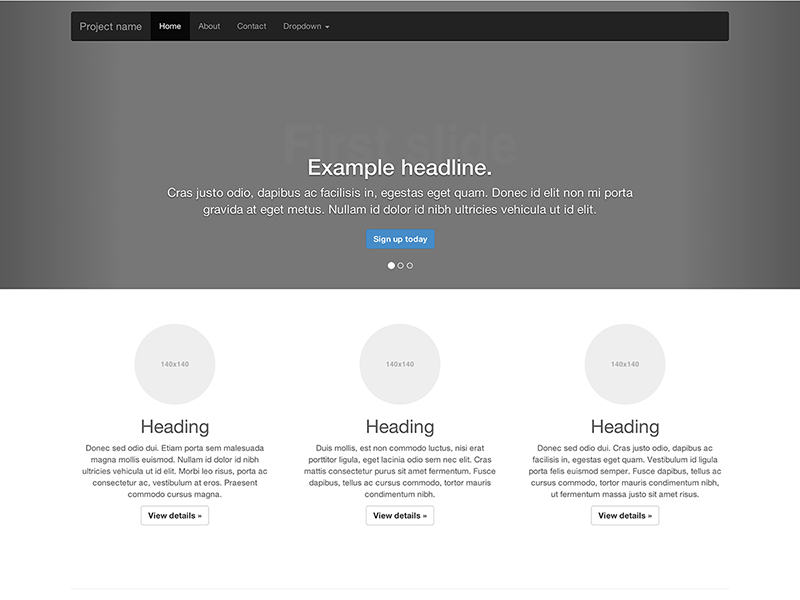
\includegraphics[scale=0.3]{img/carousel.jpg} 
\caption{Bildschirmfoto des Carousel-Templates für Bootstrap}
\label{pic:carousel}
\end{figure}
Zusätzliche Informationen über die vom Server ausgelieferten Filme fragt die Clientanwendung selbstständig durch eine Ajax-Anfrage bei der Filmdatenbank IMDB durch die kostenlose Schnittstelle \lstinline{http://www.omdbapi.com} ab. Die von dort nachgeladenen Informationen dienen nur der Information des Anwenders und fließen in keinerlei Berechnungen von Ratings oder Vergleichbarem ein.\\\\
Um die Webanwendung simpel und überschaubar zu halten, ist der Aufbau einfach strukturiert. Durch Anklicken eines Menüpunktes in der Oberfläche wird eine zugehörige JavaScript-Funktionen aufgerufen, die den für die Seite nötigen Inhalt generieren und mittels jQuery in den gewünschten Container auf der Seite angehängt (z.B. \lstinline{insertView_start()}).\\
Der gesamte Seiteninhalt befindet sich im Container \lstinline{#content-area}.\\
Wird eine weitere Seite geladen oder Inhalt mittels einer Ajax-Anfrage vom Server nachgeladen, entfernt ggf. \lstinline{clear_view()} den aktuellen Seiteninhalt und blendet einen Ladebalken ein. Sobald der erforderliche Inhalt eingetroffen ist, wird in der Callback-Funktion der Ajax-Anfrage die Funktion \lstinline{remove_loading()} aufgerufen, die sämtliche Ladebalken entfernt.

\section{Server}
Die Serveranwendung ist mit der Programmiersprache Java implementiert. Die REST-Schnittstelle wird durch das Framework \glqq Jersey\grqq\citep{lit:INET6} zur Verfügung gestellt. Als Java-basierter Webserver wird Tomcat in Version 7 verwendet.\\\\

\subsection{Statische Dateien}
Tomcat wird durch standardmäßige Webservlets in der Klasse \lstinline{com.movrec.Web_Files} angewiesen, alle Dateien des Ordners \lstinline{/MovRecTwo/src/main/resources/web} auf Anfrage auszuliefern. Der Ordner kommt demnach dem sog. \glqq Web-Root\grqq{} gleich. Um per URL an die Dateien zu gelangen, muss der Ordner \lstinline{/files/} dem Dateinamen vorangestellt werden.\\

\begin{lstlisting}[caption=Beispiel für den Aufruf einer Datei aus dem Web-Root]
http://localhost:8080/MovRecTwo/files/custom/js/movrec.js
\end{lstlisting}
%ToDo Check URL

Wird keine konkrete Datei angefordert, liefert das Servlet der Klasse \lstinline{com.movrec.Web_Index} die Datei \lstinline{index.html} aus dem Web-Root aus.


\subsection{Laden des Spark-Frameworks}
Wird die Serveranwendung gestartet, übernimmt die Klasse \lstinline{com.movrec.Web_Init} die Initalisierung des Spark-Frameworks. Die erfolgreich erstelle Instanz wird anschließend über das \glqq ServletContext\grqq{} global zur Verfügung gestellt, damit Spark durch API-Aufrufe verwendet werden kann.\\
Wird der Webserver beendet, kümmert sich die Klasse ebenfalls um die Beendigung von Spark.


\subsection{Beschreibung der REST-Schnittstelle}
Nachfolgend werden die einzelnen REST-APIs aufgeführt und deren Funktionsweise kurz erläutert.\\
Die Anfragen und Antworten sind jeweils mittels JSON formatiert.
\begin{itemize}
  \item \textbf{getRandomMovies()}\\
  	Die Funktion wird via HTTP-GET aufgerufen.\\
  	Sie liefert neun zufällig ausgewählte Filme aus dem Datenbestand zurück. Die Rückgabe enthält Key-Value Paare. Als Key definiert ist die Movie-ID aus dem Datenbestand. Das Value ist eine Liste mit den Werten Titel, Genre, IMDB-ID, Rating.\\
  	Beispiel: \lstinline{ "104177":["From One Second to the Next (2013)","Documentary","3108864","5.0"]}\\
  \item \textbf{getMoviesForRating()}\\
 	Die Funktion wird via HTTP-GET aufgerufen.\\
	Sie liefert zehn zufällig ausgewählte Filme aus dem Datenbestand zurück. Die Rückgabe enthält Key-Value Paare. Als Key definiert ist die Movie-ID aus dem Datenbestand. Das Value ist eine Liste mit den Werten Titel, Genre und IMDB-ID\\
  	Beispiel: \lstinline{ "7440":["Paper Clips (2004)","Documentary","0380615"]}\\
  \item \textbf{setMoviesForRating(@FormParam("ratingData") String ratingData)}\\
  	Die Funktion wird via HTTP-POST aufgerufen.\\
  	Als Eingabe erwartet sie Key-Value-Paare. Der Key entspricht der Movie-ID, das Value dem Rating des Nutzers zwischen 1 und 5.\\
  	Nach erfolgter Berechnung liefert sie sechs Filmvorschläge zurück. Der Key entspricht auch hier der Movie-ID, das Value einer Liste mit Titel, Genres, Rating (anderer Nutzer), Empfehlungsquote des ALS-Algorithmuses und IMDB-ID.\\
  	Beispiel: \lstinline{ "82":["Antonia's Line (Antonia) (1995)", "Comedy|Drama", "3.45", "4.090390537800163)", "0112379"]}\\
  \item \textbf{getAllGenres()}\\
  	Die Funktion wird via HTTP-GET aufgerufen.\\
  	Sie liefert alle vorkommenden Film-Genres aus dem Datenbestand zurück. Die Rückgabe enthält eine Liste mit den Genre-Bezeichnungen.\\
  	Beispiel: \lstinline{["Western","Documentary","Sci-Fi"]}\\

  \item \textbf{getMoviesForGenre(@FormParam("genre") String genre)}\\
 	Die Funktion wird via HTTP-POST aufgerufen.\\
  	Als Eingabe erwartet sie ein Key-Value-Paar. Der Key entspricht der Konstante \glqq genre\grqq, das Value den Namen des Genres.\\
  	Die Rückgabe ist analog zu \lstinline{getMoviesForRating()}.
  
\end{itemize}





\chapter{Systemkommunikation}
\label{aufbau}
\begin{figure}[htb]
\centering
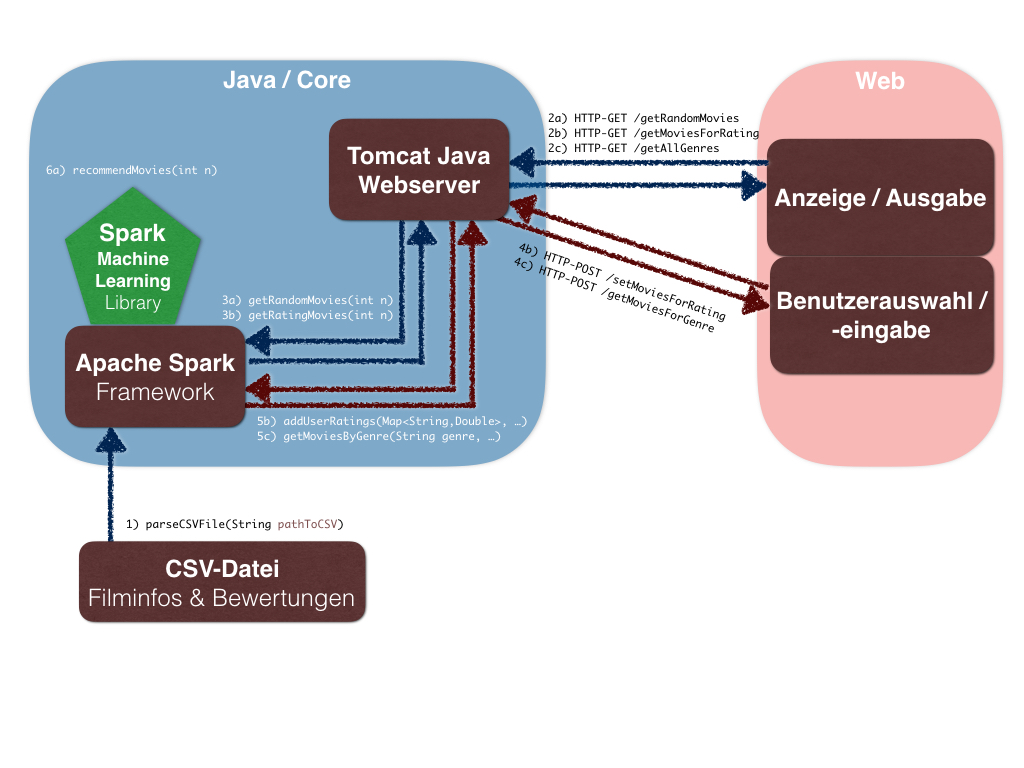
\includegraphics[scale=0.40]{img/system.jpg} 
\caption{Kommunikation im Recommendation System}
\label{pic:system}
\end{figure}
Abbildung \ref{pic:system} zeigt den geplanten Aufbau des Systems.\\
Grundlage ist ein auf Java basierender Kern, der den Zugriff auf Apache Spark und den Webserver ermöglicht. Die Machine Learning Bibliothek von Spark wird zu Beginn mit bestehenden Filmbewertungdsaten\citep{lit:INET4} trainiert. Diese werden aus einer CSV (Comma Seperated Value) Datei, welche aus dem Dateisystem gelesen wird, extrahiert.\\\\
Filminformationen und Bewertungen werden anschließend über einen in Java implementierten Webserver bereitgestellt. Der Nutzer kann sich diese somit in seinem Browser anzeigen lassen. Tätigt er eine Auswahl oder bewertet selber Filme, werden diese Informationen an den Webserver übertragen, welcher sie wiederum an Spark weiterreicht. Hier werden nun anhand der Nutzerdaten passende Vorschläge für ihn generiert und wieder über den Webserver an den Nutzer ausgeliefert.


\section{Messwerte Laufzeit}
Im folgenden werden Messwerte bezüglich der Anzahl der verwendeten Cores und der Größe der initialen Datenmenge (MovieLens\citep{lit:INET4}) tabellarisch dargestellt.\\
Zur Messung wurde Spark wie folgt konfiguriert:
\begin{lstlisting}[caption=Beispiel für Spark Setup mit zwei Cores]
SparkConf conf = new SparkConf().setAppName("Movie Recommendation");
conf.setMaster("local[2]");
sc = new JavaSparkContext(conf);
\end{lstlisting}

Die Messungen wurden unter Apple OSX 10.11.5 mit einem Intel Core i5 2,4 GHz und 8GB RAM durchgeführt.

\begin{table}[h!]
 \centering
 \caption{Messwerte}
 \label{tab:table1}
 \begin{tabular}{ccc}
   \toprule
   Cores & ml-latest-small & ml-latest\\
   \midrule
   1 & 12,986 sec * , 13,048 sec ** & 520,255 sec **\\
   2 & 17,288 sec * , 16,255 sec ** & 367,254 sec **\\
   4 & 27,456 sec * , 26,448 sec ** & 417,246 sec **\\
   \bottomrule
 \end{tabular}
\end{table}

* Alle Filme mit einem Stern bewertet;
** Alle Filme mit fünf Sternen bewertet

\newpage

%% Anhang beginnt
\appendix

%% Eidesstattliche Erklärung
%\addcontentsline{toc}{section}{Eidesstattliche Erklärung}
%%!TEX root = main.tex

%%% Text stammt von Prof. Dr. Axel Hein, Prüfungskommission, Technische Hochschule Georg Simon Ohm.

%\chapter*{}


%\thispagestyle{empty}
%\chapter*{Eidesstattliche Erklärung}
%
%\vspace*{\fill}
%Leipzig, den \today \\\\
%Ich, Matthias Frei, versichere, dass ich die Arbeit selbständig verfasst, nicht anderweitig für Prüfungszwecke vorgelegt, alle benutzten Quellen und Hilfsmittel angegeben sowie wörtliche und sinngemäße Zitate als solche gekennzeichnet habe.
%\vspace{30mm}
%\hrule
%\vspace{5mm}
%Matthias Frei
%
%\vspace*{\fill}

%\newpage


%% Ausgabe Glossar
\printglossary[style=altlist,title=Glossar,toctitle=Glossar]

%% Ausgabe des Symbolverzeichnis
% \printglossary[type=symbolslist,style=long]


%% Alle Quellen aus der bib Datei werden ins Verzeichnis aufgenommen auch wenn nicht zitiert
\nocite{*}

%%% Zweites Literaturverzeichnis z. B. für Bilder (Bildqellenverzeichnis)
%% Beachte das Flag!! Stil der Bibliographie: Nach DIN und Verzeichnis in der Reihung des Auftretens, Referenzen nummerisch
% \bibliographystyleB{unsrtdin}
%% Beachte das Flag!! Auswahl der Bib Datei. Muss die Gleiche sein wie für das normale Literaturverzeichnis!
%\bibliographyB{literatur}
%% Zitierung im Text mit \citeB{lable} Beachte Flag!!
% \renewcommand{\refname}{Bildquellenverzeichnis}

%% Stil der Bibliographie: Nach DIN und Verzeichnis in der Reihung des Auftretens, Referenzen nummerisch
\bibliographystyle{unsrtdin}

%% Stil der Bibliographie: Nach DIN und Verzeichnis sortiert (Autor, Jahr) und Vorname gekürtzt; Referenzen nummerisch
%\bibliographystyle{abbrvdin}

%% Auswahl der Bib Datei
\bibliography{literatur}

%% Index soll Stichwortverzeichnis heissen
\renewcommand{\indexname}{Stichwortverzeichnis}

%% Ausgabe des Stichwortverzeichnisses (Index)
\printindex


%%!TEX root = main.tex

% Declare new goemetry for the title page only.
%\newgeometry{left=3cm,right=2cm,top=1.5in,bottom=1in}
%---------------------------------------------

%\chapter{Statistiken der Messfahrten}
%\label{apx:stats}

%\definecolor{light-gray}{gray}{0.9}

%\lstset{
%  nolol=true,
%  numbers=left, 
%  numberstyle=\tiny, 
%  basicstyle=\ttfamily\tiny,
%  escapeinside={\%*}{*)},
%  breaklines=true,
%  tabsize=4,  
%  backgroundcolor=\color{light-gray},
%  literate=%
%    {\ \ }{{\ }}1
%    {Ö}{{\"O}}1
%    {Ä}{{\"A}}1
%    {Ü}{{\"U}}1
%    {ß}{{\ss}}1
%    {ü}{{\"u}}1
%    {ä}{{\"a}}1
%    {ö}{{\"o}}1
%    {~}{{\textasciitilde}}1
%  } 

%\section{8 KBit/s Decoder - 30/5sec Puffer}
%\lstinputlisting{appendix_files/final_8KBits_30-5sPuffer.txt}
%\newpage

% Ends the declared geometry for the titlepage
%\restoregeometry
%--------------------------
\newpage

%% Ende des Dokumenteninhalts
\end{document}